\documentclass[11pt,a4paper]{article}
\usepackage{amsmath,amssymb,amsthm}
\usepackage[margin=2.5cm]{geometry}
\usepackage{hyperref}

\newtheorem{theorem}{Theorem}
\newtheorem{lemma}[theorem]{Lemma}
\newtheorem{proposition}[theorem]{Proposition}
\newtheorem{corollary}[theorem]{Corollary}
\theoremstyle{definition}
\newtheorem{definition}[theorem]{Definition}
\newtheorem{remark}[theorem]{Remark}
\newtheorem{example}[theorem]{Example}

\newcommand{\R}{\mathbb{R}}
\newcommand{\sa}{\mathrm{sa}}
\newcommand{\aff}{\operatorname{aff}}
\newcommand{\spn}{\operatorname{span}}
\newcommand{\face}{\operatorname{face}}
\newcommand{\rank}{\operatorname{rank}}
\newcommand{\PSD}{\mathrm{PSD}}
\newcommand{\Sym}{\mathrm{Sym}}
\newcommand{\tr}{\operatorname{tr}}
\newcommand{\im}{\operatorname{im}}
\newcommand{\id}{\mathbf{1}}
\newcommand{\Tr}{\operatorname{Tr}}
\newcommand{\ket}[1]{|#1\rangle}
\newcommand{\bra}[1]{\langle#1|}
\newcommand{\braket}[2]{\langle#1|#2\rangle}
\usepackage{booktabs}
\usepackage{pgfplots}
\pgfplotsset{compat=newest}
\usepgfplotslibrary{groupplots}
\usetikzlibrary{patterns}
\pgfplotsset{
    table/.append style={col sep=space, header=true},
}

\title{A Barvinok--Pataki Theorem for Archimedean Order Unit Spaces}
\author{Timo Ziegler,$^{1}$
  Tobias J.\ Osborne,$^{1}$
  Martin Plavala,$^{2}$ \\
  Ren\'e Schwonnek,$^{1}$
  Lennart Binkowski,$^{1}$
  Lukas Hantzko,$^{2}$ \\
  Henrik Wilming,$^{1}$
  Alexander Stottmeister$^{3}$ \\[6pt]
  \small $^1$AG Osborne, Institut f\"ur Theoretische Physik,
    Leibniz Universit\"at Hannover \\
  \small $^2$AG Raussendorf, Institut f\"ur Theoretische Physik,
    Leibniz Universit\"at Hannover \\
  \small $^3$Quantum Information Group, Institut f\"ur Theoretische Physik,
    Leibniz Universit\"at Hannover \\[4pt]
  \small Based on a blackboard discussion, 3 March 2026}
\date{}

\begin{document}
\maketitle

\begin{abstract}
We prove a generalisation of the Barvinok--Pataki rank bound to
Archimedean order unit spaces equipped with a pointed cone.  The
classical result bounds the rank of extreme points of spectrahedra
(feasible sets of semidefinite programs); our generalisation bounds the
face dimension of feasible points under affine constraints in an
arbitrary pointed cone, including the infinite-dimensional case.
The face-dimension bound $d_F \leq m$ uses only pointedness of the
cone and rank--nullity; finite-dimensionality of $d_F$ in infinite
dimensions follows from a result of Weis--Shirokov that requires
only a real vector space and a convex set.  When specialised to
C$^*$-algebras via the Alfsen--Shultz face--commutant correspondence,
this recovers the operator-algebraic Barvinok--Pataki bound
$\sum n_j^2 \leq m + 1$.
\end{abstract}

%% ========================================================================
\section{Preliminaries}
%% ========================================================================

\begin{definition}[Ordered vector space with cone]
Let $V$ be a real vector space.  A \emph{cone} is a subset
$V^+ \subseteq V$ that is closed under addition and non-negative
scalar multiplication.  The pair $(V, V^+)$ is an \emph{ordered
vector space} with partial order $x \leq y$ iff $y - x \in V^+$.
\end{definition}

\begin{definition}[Pointed cone]
A cone $V^+$ is \emph{pointed} (or \emph{proper}) if
$V^+ \cap (-V^+) = \{0\}$, i.e.\ the only element $v$ with both
$v \geq 0$ and $-v \geq 0$ is $v = 0$.
\end{definition}

\begin{definition}[Order unit and Archimedean property]
An element $e \in V^+$ is an \emph{order unit} if for every $v \in V$
there exists $n \in \mathbb{N}$ such that $ne - v \in V^+$ (i.e.\
$v \leq ne$).  The cone $V^+$ is \emph{Archimedean} if, whenever
$ne + v \in V^+$ for all $n \in \mathbb{N}$, it follows that
$v \in V^+$.  The triple $(V, V^+, e)$ is called an \emph{Archimedean
order unit space} (AOU space).
\end{definition}

\begin{definition}[Face of a cone]\label{def:face}
Let $V^+$ be a cone in $V$ and $x \in V^+$.  The \emph{face of $V^+$
generated by $x$} is
\[
  \face_{V^+}(x)
  \;=\;
  \bigl\{\, w \in V^+ \;\big|\;
    \exists\, \lambda > 0 \colon x - \lambda w \in V^+ \,\bigr\}.
\]
Equivalently, $\face_{V^+}(x)$ consists of all elements of $V^+$ that
can be ``majorised'' by a positive multiple of $x$.  This is the
smallest face of $V^+$ containing $x$ in its relative interior.
\end{definition}

\begin{remark}
In a pointed cone, $\face_{V^+}(x) = \{0\}$ if and only if $x = 0$.
For $x \neq 0$, the face is at least one-dimensional (it contains
the ray $\{\lambda x : \lambda \geq 0\}$).  For the PSD cone
$\PSD_n$, the face generated by a rank-$r$ matrix $X$ is
isomorphic to $\PSD_r$, with
$\dim(\face(X)) = \frac{r(r+1)}{2}$ (real symmetric case) or
$r^2$ (complex Hermitian case).
\end{remark}

%% ========================================================================
\section{The Classical Barvinok--Pataki Bound}
%% ========================================================================

We first recall the classical proof for PSD matrices, as it motivates
each step of the generalisation.

\begin{theorem}[Barvinok--Pataki, PSD case]\label{thm:classical}
Let $A_1, \dots, A_m \in \Sym_n(\R)$ and $\beta_1, \dots, \beta_m \in \R$.
Consider the spectrahedron
\[
  C = \bigl\{\, X \in \PSD_n \;\big|\;
    \langle A_j, X \rangle = \beta_j,\; j = 1, \dots, m \,\bigr\}.
\]
If $X \in C$ is an extreme point of $C$, then
$\frac{r(r+1)}{2} \leq m$ where $r = \rank(X)$.
\end{theorem}

\begin{proof}
Write $X = V B V^\top$ with $V \in \R^{n \times r}$,
$B \in \PSD_r$ strictly positive definite.
Define the compressed constraints $\hat{A}_j = V^\top A_j V \in \Sym_r$
and the linear map
\[
  \varphi \colon \Sym_r \to \R^m, \qquad
  [\varphi(D)]_j = \langle \hat{A}_j, D \rangle.
\]
By rank--nullity, $\dim(\ker\varphi) \geq \frac{r(r+1)}{2} - m$.
If $\ker\varphi \neq \{0\}$, choose $D \neq 0$ in $\ker\varphi$.
Then $B(t) = B + tD$ satisfies all constraints for every $t$.

Since $B \succ 0$ and $D$ is a non-zero symmetric matrix with at least
one negative eigenvalue (replacing $D$ by $-D$ if necessary), the map
$t \mapsto \lambda_{\min}(B + tD)$ is continuous, positive at $t = 0$,
and decreasing for $t > 0$.  Let $t_0 > 0$ be the first value where
$\lambda_{\min}(B + t_0 D) = 0$.  Then $B(t_0) \succeq 0$ with
$\rank(B(t_0)) < r$, and $V B(t_0) V^\top \in C$.

This contradicts $X$ being an extreme point of $C$ (since $X$ is a
non-trivial convex combination of $V B(t_0) V^\top$ and
$V B(-t_0') V^\top$ for suitably chosen $t_0'$), unless
$\ker\varphi = \{0\}$, which forces $\frac{r(r+1)}{2} \leq m$.
\end{proof}

%% ========================================================================
\section{Generalisation to Pointed Cones}
%% ========================================================================

The key observation is that the proof above uses only three ingredients:
\begin{enumerate}
\item \textbf{Rank--nullity} for the constraint map restricted to the
  face;
\item \textbf{Pointedness} of the cone, to guarantee that a line
  through an interior point of a face must exit the cone;
\item \textbf{Finite-dimensionality} of the face, to apply
  rank--nullity with finite dimensions.
\end{enumerate}

\begin{theorem}[Barvinok--Pataki for pointed cones]\label{thm:general}
Let $V$ be a real vector space, $V^+\subseteq V$ a pointed cone, and
$\alpha_1, \dots, \alpha_m \in V^*$ linear functionals.  Define
\[
  C = \bigl\{\, x \in V^+ \;\big|\;
    \alpha_j(x) = b_j,\; j = 1, \dots, m \,\bigr\}
\]
for given $b_1, \dots, b_m \in \R$.  Let $x \in C$ and let
$F = \face_{V^+}(x)$ be the face of $V^+$ generated by $x$.
Assume that $d_F := \dim(\spn(F))$ is finite.  Define the restricted
constraint map
\[
  \varphi_F \colon \spn(F) \to \R^m, \qquad
  [\varphi_F(v)]_j = \alpha_j(v).
\]
If $x$ is an extreme point of $C$, then
\[
  \boxed{\; d_F \;\leq\; m. \;}
\]
Equivalently, $\dim(F) \leq m - 1$ (where $\dim(F)$ is the dimension
of $F$ as a convex set, i.e.\ $\dim(\aff(F))$).
\end{theorem}

\begin{proof}
By rank--nullity applied to $\varphi_F$,
\[
  d_F
  \;=\; \dim(\ker \varphi_F) + \dim(\im \varphi_F)
  \;\leq\; \dim(\ker \varphi_F) + m.
\]
It suffices to show that $\ker\varphi_F = \{0\}$ when $x$ is extreme
in $C$.  Suppose for contradiction that there exists
$D \in \ker\varphi_F$, $D \neq 0$.

\medskip
\noindent\textbf{Step 1: The perturbation preserves feasibility.}
Since $D \in \spn(F) \cap \ker\varphi_F$, we have
$\alpha_j(D) = 0$ for all $j$.  Therefore, for any $t \in \R$:
\[
  \alpha_j(x + tD) = \alpha_j(x) + t \,\alpha_j(D) = b_j.
\]
So $x + tD$ satisfies all affine constraints whenever it lies in $V^+$.

\medskip
\noindent\textbf{Step 2: Pointedness forces exit from the cone.}
Since $V^+$ is pointed, we cannot have both $D \in V^+$ and
$-D \in V^+$ (this would imply $D = 0$).  Therefore, at least one of
the half-lines $\{x + tD : t > 0\}$ or $\{x - tD : t > 0\}$ must
eventually leave $V^+$.

More precisely: since $x$ lies in the relative interior of $F$, for
sufficiently small $|t|$ we have $x + tD \in F \subseteq V^+$ (as
$D \in \spn(F)$ and $x$ is an interior point of $F$).  But the line
cannot remain in $V^+$ in both directions indefinitely, since this
would imply $D$ and $-D$ are both in $V^+$ (by rescaling), contradicting
pointedness.

\medskip
\noindent\textbf{Step 3: Walking to a smaller face.}
Let
\[
  t^+ = \sup\{t > 0 : x + tD \in V^+\}, \qquad
  t^- = \sup\{t > 0 : x - tD \in V^+\}.
\]
By Step~2, at least one of $t^+$, $t^-$ is finite.  Say
$t^+ < \infty$ (the other case is symmetric).

If $V^+$ is closed (which holds in finite dimensions, or under the
Archimedean assumption in the norm topology), then
$x^* := x + t^+ D \in V^+$, and $x^*$ lies on the boundary of $V^+$
relative to $\spn(F)$.  This means $x^*$ belongs to a \emph{proper
face} $F' \subsetneq F$, so $\dim(F') < \dim(F)$.  Moreover, $x^*$
satisfies all constraints, so $x^* \in C$.

\medskip
\noindent\textbf{Step 4: Contradiction with extremality.}
We have $x^* = x + t^+ D \in C$ and (if $t^- > 0$, which holds since
$x$ is interior to $F$) also $x^{**} = x - \varepsilon D \in C$ for
small $\varepsilon > 0$.  Then
\[
  x = \frac{\varepsilon}{t^+ + \varepsilon}\, x^*
    + \frac{t^+}{t^+ + \varepsilon}\, x^{**},
\]
exhibiting $x$ as a non-trivial convex combination of two distinct
elements of $C$.  If $x$ were an extreme point of $C$, this is a
contradiction.

Therefore $\ker\varphi_F = \{0\}$, and we conclude $d_F \leq m$.
\end{proof}

%% ========================================================================
\section{Application to C$^*$-Algebras and AOU Spaces}
%% ========================================================================

\begin{corollary}[Barvinok--Pataki for AOU spaces]\label{cor:aou}
Let $(V, V^+, e)$ be an Archimedean order unit space with
$\dim(V) < \infty$.  Let $\alpha_1, \dots, \alpha_m \in V^*$ and
consider the state-like set
\[
  C = \bigl\{\, x \in V^+ \;\big|\;
    \alpha_j(x) = b_j,\; j = 1, \dots, m \,\bigr\}.
\]
For any extreme point $x$ of $C$, the face of $V^+$ generated by $x$
satisfies $\dim(\face_{V^+}(x)) \leq m - 1$.
\end{corollary}

\begin{proof}
The Archimedean property implies the cone $V^+$ is closed (in the
order-unit norm) and pointed.  In finite dimensions, every face
is finite-dimensional.  Apply Theorem~\ref{thm:general}.
\end{proof}

\begin{corollary}[Barvinok--Pataki for C$^*$-algebras]\label{cor:cstar}
Let $A$ be a unital C$^*$-algebra and $a_1, \dots, a_m \in A_\sa$.
Consider the affinely constrained state space
\[
  C = \bigl\{\, \varphi \in S(A) \;\big|\;
    \varphi(a_j) = \beta_j,\; j = 1, \dots, m \,\bigr\},
\]
where $S(A) = \{\varphi \in A^* : \varphi \geq 0,\, \varphi(\id) = 1\}$.
If $\varphi$ is an extreme point of $C$, then
\[
  \dim_\R\bigl(\pi_\varphi(A)'\bigr)_\sa \;\leq\; m + 1,
\]
where $\pi_\varphi$ is the GNS representation of $\varphi$.
Equivalently, if $\pi_\varphi(A)' \cong \bigoplus_j M_{n_j}(\mathbb{C})$
(Artin--Wedderburn), then $\sum_j n_j^2 \leq m + 1$.
\end{corollary}

\begin{proof}
The state space $S(A)$ is a base for the cone $A^*_+$ (positive
functionals), cut out by the normalisation constraint
$\varphi(\id) = 1$.  The total number of affine constraints on
$A^*_+$ is $m + 1$ (the $m$ given constraints plus normalisation).

By the Alfsen--Shultz face--commutant correspondence, the face
of $S(A)$ generated by $\varphi$ is affinely isomorphic to the state
space $S(\pi_\varphi(A)')$ of the commutant.  In particular,
\[
  \dim\bigl(\face_{S(A)}(\varphi)\bigr)
  = \dim_\R\bigl(\pi_\varphi(A)'\bigr)_\sa - 1.
\]
Applying Theorem~\ref{thm:general} with the $m + 1$ constraints on
$A^*_+$ gives $\dim(\spn(\face(\varphi))) \leq m + 1$, hence
$\dim_\R(\pi_\varphi(A)')_\sa \leq m + 1$.
\end{proof}

%% ========================================================================
\section{The Infinite-Dimensional Case and the Role of $d_F$}
\label{sec:infinite-dim}
%% ========================================================================

Theorem~\ref{thm:general} assumes that $d_F = \dim(\spn(F))$ is
finite.  In infinite dimensions this is a non-trivial hypothesis:
the face of a cone generated by a point can be
infinite-dimensional.  We now show that this hypothesis is
\emph{automatically satisfied} whenever the number of constraints
is finite, using a result of Weis--Shirokov that is purely
convex-geometric.

\begin{theorem}[Weis--Shirokov {\cite[Theorem~3.3]{weis_shirokov21}}]
\label{thm:ws}
Let $V$ be a real vector space, $K \subseteq V$ a convex set, and
$f \colon K \to \R \cup \{+\infty\}$ a generalised affine map.
Let $C$ denote a sublevel set $\{x \in K : f(x) \leq \alpha\}$
or a level set $\{x \in K : f(x) = \alpha\}$, and let $x \in C$.
If the face $F_C(x)$ of $C$ generated by $x$ has dimension
$m \in \mathbb{N}_0$, then the face $F_K(x)$ of $K$ generated by
$x$ has dimension $m$ or $m + 1$.
\end{theorem}

The multi-constraint version follows by induction (Corollary~5 of
\cite{weis_shirokov21}): if $C$ is the intersection of $\ell$
sublevel and/or level sets of generalised affine maps, and
$F_C(x)$ has dimension $m$, then
$\dim(F_K(x)) \in \{m, m+1, \ldots, m + \ell\}$.

\begin{corollary}[Finiteness of $d_F$]\label{cor:dF-finite}
Let $K$ be a convex set in a real vector space $V$, and let $C$ be
defined by $\ell$ generalised affine constraints on $K$.  If $x$
is an extreme point of $C$, then
\[
  \dim\bigl(F_K(x)\bigr) \;\leq\; \ell.
\]
In particular, the face of $K$ generated by any extreme point of
$C$ is finite-dimensional, regardless of $\dim(V)$.
\end{corollary}

\begin{proof}
Since $x$ is extreme in $C$, the face $F_C(x) = \{x\}$ has
dimension~$0$.  By the multi-constraint version of
Theorem~\ref{thm:ws}, $\dim(F_K(x)) \in \{0, 1, \ldots, \ell\}$.
\end{proof}

\begin{remark}[No operator-algebraic assumptions needed]
\label{rmk:no-opalg}
Theorem~\ref{thm:ws} and Corollary~\ref{cor:dF-finite} require
only a real vector space $V$ and a convex subset $K \subseteq V$.
In particular:
\begin{itemize}
\item No cone structure, pointedness, or Archimedean property is
  needed to establish that $d_F$ is finite.
\item No C$^*$-algebraic or operator-algebraic notions are needed.
\item The operator-algebraic machinery (GNS representation,
  face--commutant correspondence, Artin--Wedderburn decomposition)
  is used only in a second step: to \emph{interpret} the
  finite-dimensional face algebraically as a commutant and extract
  the multiplicity bound $\sum n_j^2 \leq m + 1$.
\end{itemize}
This clarifies the logical structure of the infinite-dimensional
case: Weis--Shirokov provides the purely geometric bound on $d_F$,
and the Alfsen--Shultz correspondence translates it into algebra.
\end{remark}

Combining Corollary~\ref{cor:dF-finite} with
Theorem~\ref{thm:general}, we obtain the following
infinite-dimensional version of the main theorem that does not
require an a priori finiteness assumption on $d_F$.

\begin{corollary}[Barvinok--Pataki for infinite-dimensional
pointed cones]\label{cor:inf-dim}
Let $V$ be a (possibly infinite-dimensional) real vector space,
$V^+ \subseteq V$ a pointed closed cone, and
$\alpha_1, \ldots, \alpha_m \in V^*$ linear functionals.  Define
$C = \{x \in V^+ : \alpha_j(x) = b_j\}$.  If $x$ is an extreme
point of $C$, then
\[
  d_F = \dim\bigl(\spn(\face_{V^+}(x))\bigr) \leq m.
\]
\end{corollary}

\begin{proof}
By Corollary~\ref{cor:dF-finite} (with $K = V^+$ viewed as a
convex set and $\ell = m$), $d_F$ is finite.
Theorem~\ref{thm:general} then gives $d_F \leq m$.
\end{proof}

%% ========================================================================
\section{Special Cases Recovered}
%% ========================================================================

\begin{enumerate}
\item \textbf{Classical Barvinok--Pataki} ($A = M_n(\mathbb{C})$).
  The unique irreducible representation is the identity, so
  $\pi_\varphi(A)' \cong M_r(\mathbb{C})$ where $r = \rank(\rho_\varphi)$.
  Hence $r^2 \leq m + 1$, or $r^2 \leq m$ when one of the constraints
  is the trace normalisation already built into the spectrahedron.

\item \textbf{Carath\'eodory's theorem} ($A = C(X)$, abelian).
  All irreducible representations are one-dimensional, so the commutant
  decomposes as $\bigoplus_{j=1}^k \mathbb{C}$.  The bound gives
  $k \leq m + 1$: extreme measures under $m$ moment constraints are
  supported on at most $m + 1$ points.

\item \textbf{Block-diagonal algebras} ($A = \bigoplus_i M_{d_i}(\mathbb{C})$).
  The bound $\sum_i r_i^2 \leq m + 1$ simultaneously constrains ranks
  within blocks \emph{and} the number of active blocks.

\item \textbf{Infinite-dimensional} ($A = B(\mathcal{H})$).
  For normal states (density operators) under $m$ constraints
  (including possibly unbounded Hamiltonians, handled via the
  Weis--Shirokov framework): $r^2 \leq m + 1$.  In particular,
  $m \leq 2$ constraints imply all extreme points are pure states.
\end{enumerate}

%% ========================================================================
\section{Physical Example: Hydrogen Atom in a Magnetic Field}
\label{sec:hydrogen}
%% ========================================================================

We illustrate the theorem with a concrete physical system: the
hydrogen atom in an external magnetic field, subject to angular
momentum constraints.  This example demonstrates how the
Barvinok--Pataki bound determines when pure-state variational
methods suffice and when mixed states are unavoidable.

\subsection{Hilbert space and quantum numbers}

The non-relativistic hydrogen atom has Hilbert space
$\mathcal{H} = L^2(\R^3) \otimes \mathbb{C}^2$ (spatial wave function
tensored with spin-$\tfrac{1}{2}$).  The Coulomb Hamiltonian
\[
  H_0 = -\frac{\hbar^2}{2m_e}\nabla^2 - \frac{e^2}{4\pi\varepsilon_0\, r}
\]
has eigenvalues $E_n = -13.6\;\mathrm{eV}/n^2$ for $n = 1, 2, 3, \ldots$,
with simultaneous eigenstates $\ket{n, l, m_l, m_s}$ labelled by:
\begin{center}
\begin{tabular}{lll}
\toprule
\textbf{Quantum number} & \textbf{Range} & \textbf{Observable} \\
\midrule
$n$ (principal) & $1, 2, 3, \ldots$ & $H_0$ (energy) \\
$l$ (orbital ang.\ mom.) & $0, 1, \ldots, n - 1$ & $\mathbf{L}^2 = l(l+1)\hbar^2$ \\
$m_l$ (magnetic) & $-l, -l+1, \ldots, l$ & $L_z = m_l \hbar$ \\
$m_s$ (spin) & $\pm\tfrac{1}{2}$ & $S_z = m_s \hbar$ \\
\bottomrule
\end{tabular}
\end{center}
The degeneracy of the $n$-th energy shell is $g_n = 2n^2$ (including
spin).  The total angular momentum is $\mathbf{J} = \mathbf{L} + \mathbf{S}$,
with $J_z = L_z + S_z$ having eigenvalue $m_j \hbar$ where $m_j = m_l + m_s$.

\subsection{Zeeman Hamiltonian}

In a uniform magnetic field $\mathbf{B} = B\hat{z}$, the interaction
Hamiltonian is
\[
  H_Z = \frac{\mu_B B}{\hbar}\bigl(L_z + g_s\, S_z\bigr),
\]
where $\mu_B = e\hbar/(2m_e)$ is the Bohr magneton and $g_s \approx 2$
is the electron spin $g$-factor.  On the standard basis,
$H_Z \ket{n,l,m_l,m_s} = \mu_B B (m_l + 2m_s)\ket{n,l,m_l,m_s}$.
The full Hamiltonian is $H = H_0 + H_Z$.

\subsection{The constrained optimisation problem}

We seek the state of minimum energy subject to a constraint on the
total angular momentum projection:
\begin{equation}\label{eq:hydrogen-opt}
  \min_{\rho}\; \Tr(H\rho)
  \qquad\text{subject to}\qquad
  \rho \geq 0, \;\; \Tr(\rho) = 1, \;\;
  \Tr(J_z\, \rho) = M\hbar.
\end{equation}
This is a convex optimisation (linear objective over a convex
constraint set).  The minimum is attained at an extreme point of the
feasible set
\[
  C = \bigl\{\rho \in \mathfrak{S}(\mathcal{H}) :
  \Tr(J_z\,\rho) = M\hbar\bigr\},
\]
where $\mathfrak{S}(\mathcal{H})$ is the set of density operators on
$\mathcal{H}$.

\subsection{Applying the Barvinok--Pataki bound}

\paragraph{Full Hilbert space ($A = B(\mathcal{H})$, infinite-dimensional).}

The constraint $\Tr(J_z\,\rho) = M\hbar$ constitutes $m = 1$ affine
constraint on the state space $\mathfrak{S}(\mathcal{H})$.  By
Corollary~\ref{cor:cstar} (or Corollary~\ref{cor:inf-dim} applied to
the positive cone in the trace-class operators),
\[
  r^2 \;\leq\; m + 1 = 2,
  \qquad\text{hence}\qquad r = 1.
\]
\emph{The energy minimiser is a pure state.}

More generally, with $m$ constraints:
\begin{center}
\begin{tabular}{clcl}
\toprule
$m$ & \textbf{Constraints} & \textbf{Rank bound} & \textbf{Conclusion} \\
\midrule
1 & $\Tr(J_z\,\rho) = M\hbar$ & $r = 1$ & Pure state \\
2 & $+ \;\Tr(\mathbf{J}^2\,\rho) = j(j+1)\hbar^2$ & $r = 1$ & Pure state \\
3 & $+ \;\Tr(\mathbf{L}^2\,\rho) = l(l+1)\hbar^2$ & $r \leq 2$ & Rank $\leq 2$ \\
4 & $+ \;\Tr(H_0\,\rho) = E$ & $r \leq 2$ & Rank $\leq 2$ \\
\bottomrule
\end{tabular}
\end{center}
The transition from pure to potentially mixed occurs at $m = 3$: this
is a direct consequence of the face dimension gap for
$B(\mathcal{H})$, which has $\{1, 2\} \subseteq G(B(\mathcal{H}))$
(the face dimension spectrum is $\{0, 3, 8, 15, \ldots\}$).

\paragraph{Restriction to the $n = 2$ shell.}

For a concrete finite-dimensional calculation, restrict to the
$n = 2$ shell.  This has $g_2 = 2 \cdot 4 = 8$ states, so
$\mathcal{H}_{n=2} \cong \mathbb{C}^8$ and $A = M_8(\mathbb{C})$:
\begin{center}
\begin{tabular}{cccccc}
\toprule
$l$ & $m_l$ & $m_s$ & $m_j = m_l + m_s$ & $m_l + 2m_s$ & \textbf{Subshell} \\
\midrule
0 & $0$   & $+\tfrac{1}{2}$ & $+\tfrac{1}{2}$ & $1$ & $2s$ \\
0 & $0$   & $-\tfrac{1}{2}$ & $-\tfrac{1}{2}$ & $-1$ & $2s$ \\
1 & $-1$  & $+\tfrac{1}{2}$ & $-\tfrac{1}{2}$ & $0$ & $2p$ \\
1 & $-1$  & $-\tfrac{1}{2}$ & $-\tfrac{3}{2}$ & $-2$ & $2p$ \\
1 & $0$   & $+\tfrac{1}{2}$ & $+\tfrac{1}{2}$ & $1$ & $2p$ \\
1 & $0$   & $-\tfrac{1}{2}$ & $-\tfrac{1}{2}$ & $-1$ & $2p$ \\
1 & $1$   & $+\tfrac{1}{2}$ & $+\tfrac{3}{2}$ & $2$ & $2p$ \\
1 & $1$   & $-\tfrac{1}{2}$ & $+\tfrac{1}{2}$ & $0$ & $2p$ \\
\bottomrule
\end{tabular}
\end{center}
The Coulomb Hamiltonian is $H_0 = E_2\, I_8$ (degenerate on the
shell).  Including spin--orbit coupling (fine structure),
$H_{\mathrm{fs}} = \xi_{21}\,\mathbf{L}\cdot\mathbf{S}$ splits the
shell into multiplets: $2s_{1/2}$ ($l = 0$, $j = \tfrac{1}{2}$, 2
states), $2p_{1/2}$ ($l = 1$, $j = \tfrac{1}{2}$, 2 states), and
$2p_{3/2}$ ($l = 1$, $j = \tfrac{3}{2}$, 4 states).  The Zeeman
term $H_Z = \mu_B B (m_l + 2m_s)$ is diagonal in the
$\ket{l, m_l, m_s}$ basis.

The optimisation \eqref{eq:hydrogen-opt} restricted to this shell is
an SDP on $M_8(\mathbb{C})$.  Normalisation $\Tr(\rho) = 1$ is built
into the state space.  The Barvinok--Pataki bound gives:
\begin{center}
\begin{tabular}{clcc}
\toprule
$m$ & \textbf{Constraints (on the $n=2$ shell)} & $r^2 \leq m + 1$
& \textbf{Na\"{\i}ve bound} \\
\midrule
1 & $\Tr(J_z\,\rho) = M\hbar$ & $r = 1$ & $r \leq 8$ \\
2 & $+\;\Tr(\mathbf{J}^2\,\rho) = j(j+1)\hbar^2$ & $r = 1$ & $r \leq 8$ \\
3 & $+\;\Tr(\mathbf{L}^2\,\rho) = l(l+1)\hbar^2$ & $r \leq 2$ & $r \leq 8$ \\
5 & $+\;\Tr(S_z\,\rho) = s\hbar,\; \Tr(L_z\,\rho) = \mu\hbar$ & $r \leq 2$
& $r \leq 8$ \\
\bottomrule
\end{tabular}
\end{center}

\subsection{Physical interpretation}

\begin{enumerate}
\item \textbf{Automatic purity ($m \leq 2$).}  Fixing the total
  angular momentum projection $M$ (and optionally $j$) is enough to
  guarantee that the energy minimiser is a pure state.  This means
  pure-state variational methods (e.g.\ Rayleigh--Ritz, DMRG for the
  ground state) are \emph{exact} for this problem --- there is no
  advantage to working with density matrices.

\item \textbf{Low-rank mixed states ($m = 3$).}  Adding a third
  constraint (e.g.\ fixing $l$) opens the door to rank-$2$ optimisers:
  the energy minimiser may be a \emph{statistical mixture} of two pure
  states.  But the rank is at most~2, not~8; thus only a
  two-dimensional search is needed, rather than optimisation over all
  $8 \times 8$ density matrices.

  This bound is \textbf{tight}: when the constraint values lie in
  the interior of the joint numerical range --- i.e.\ values not
  achievable by any single pure state --- the optimizer is genuinely
  mixed.  For example, on the $n = 2$ shell with $m = 3$ constraints
  $\langle J_z \rangle = 0$, $\langle \mathbf{J}^2 \rangle = 2$,
  $\langle \mathbf{L}^2 \rangle = 1$ (values strictly between the
  eigenvalues of $\mathbf{J}^2$), the SDP optimizer has
  $\rank(\rho^*) = 2$ with eigenvalues
  $(\lambda_1, \lambda_2) \approx (0.569, 0.431)$.  See
  Table~\ref{tab:rank2} and Figure~\ref{fig:rank2-eigs}.

\item \textbf{Practical consequence.}  For a numerical SDP solving
  \eqref{eq:hydrogen-opt}, interior-point methods converge to the
  analytic centre (maximal rank), but the theorem guarantees that
  facial reduction or rank minimisation will find a solution of rank
  $\leq \lfloor\sqrt{m+1}\rfloor$.  This dramatically reduces the
  dimension of the search space: on the $n = 3$ shell ($g_3 = 18$,
  $\rho \in M_{18}(\mathbb{C})$), even $m = 10$ constraints yield
  $r \leq 3$ rather than $r \leq 18$.
\end{enumerate}

\begin{table}[htbp]
\centering
\caption{Genuine rank-$2$ optimizers on hydrogen shells with $m = 3$
constraints (BP bound $r \leq 2$).  Constraint values are chosen in
the interior of the joint numerical range, where no pure state is
feasible.}
\label{tab:rank2}
\begin{tabular}{cccccccc}
\toprule
$n$ & $\dim$ & $\langle J_z\rangle$ & $\langle \mathbf{J}^2\rangle$
& $\langle \mathbf{L}^2\rangle$ & $\rank$ & $\lambda_1$ & $\lambda_2$ \\
\midrule
2 & 8  & $0$   & $2.0$ & $1.0$ & $\mathbf{2}$ & $0.569$ & $0.431$ \\
2 & 8  & $0$   & $1.5$ & $0.5$ & $\mathbf{2}$ & $0.754$ & $0.246$ \\
3 & 18 & $0$   & $4.0$ & $3.0$ & $\mathbf{2}$ & $0.675$ & $0.325$ \\
\bottomrule
\end{tabular}
\end{table}

\begin{figure}[htbp]
\centering
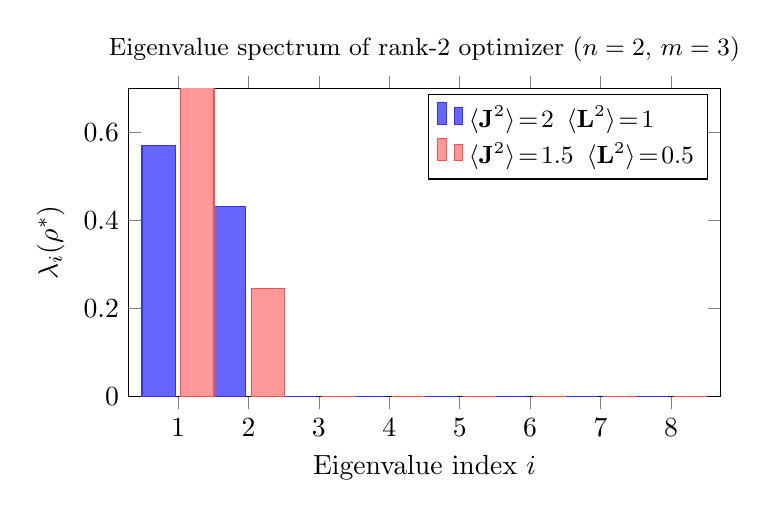
\begin{tikzpicture}
\begin{axis}[
    ybar,
    /pgf/bar width=12pt,
    width=0.75\textwidth,
    height=5.5cm,
    xlabel={Eigenvalue index $i$},
    ylabel={$\lambda_i(\rho^*)$},
    ymin=0, ymax=0.7,
    xtick={1,2,3,4,5,6,7,8},
    legend style={at={(0.98,0.98)}, anchor=north east, font=\small},
    legend cell align=left,
    title={Eigenvalue spectrum of rank-$2$ optimizer ($n=2$, $m=3$)},
    title style={font=\small},
]
\addplot[fill=blue!60, draw=blue!80] coordinates {
    (1, 0.569) (2, 0.431) (3, 0.0) (4, 0.0) (5, 0.0) (6, 0.0) (7, 0.0) (8, 0.0)
};
\addplot[fill=red!40, draw=red!70] coordinates {
    (1, 0.754) (2, 0.246) (3, 0.0) (4, 0.0) (5, 0.0) (6, 0.0) (7, 0.0) (8, 0.0)
};
\legend{$\langle\mathbf{J}^2\rangle\!=\!2$\, $\langle\mathbf{L}^2\rangle\!=\!1$,
        $\langle\mathbf{J}^2\rangle\!=\!1.5$\, $\langle\mathbf{L}^2\rangle\!=\!0.5$}
\end{axis}
\end{tikzpicture}
\caption{Eigenvalue spectra of two genuine rank-$2$ optimizers on the
$n=2$ shell ($\dim=8$) with $m=3$ constraints and
$\langle J_z \rangle = 0$.  Exactly two eigenvalues are non-zero,
saturating the BP bound $r \leq \lfloor\sqrt{m+1}\rfloor = 2$.
The constraint values lie in the interior of the joint numerical range
and cannot be achieved by any pure state.}
\label{fig:rank2-eigs}
\end{figure}

\subsection{Numerical verification}

We verified the Barvinok--Pataki bound numerically by solving the SDP
\eqref{eq:hydrogen-opt} using the Mosek interior-point solver (via
JuMP in Julia) for hydrogen shells $n = 2, 3, 4, 5$
($\dim = 8, 18, 32, 50$), field strengths $B \in [0.05, 5]$, and
$m = 0, \ldots, 5$ angular momentum constraints.  A two-phase
approach was used: Phase~1 finds the optimal energy $E^*$; Phase~2
adds a small random Hermitian perturbation to the objective while
pinning $\Tr(H\rho) = E^*$, generically selecting a unique extreme
point of the optimal face.

\begin{figure}[htbp]
\centering
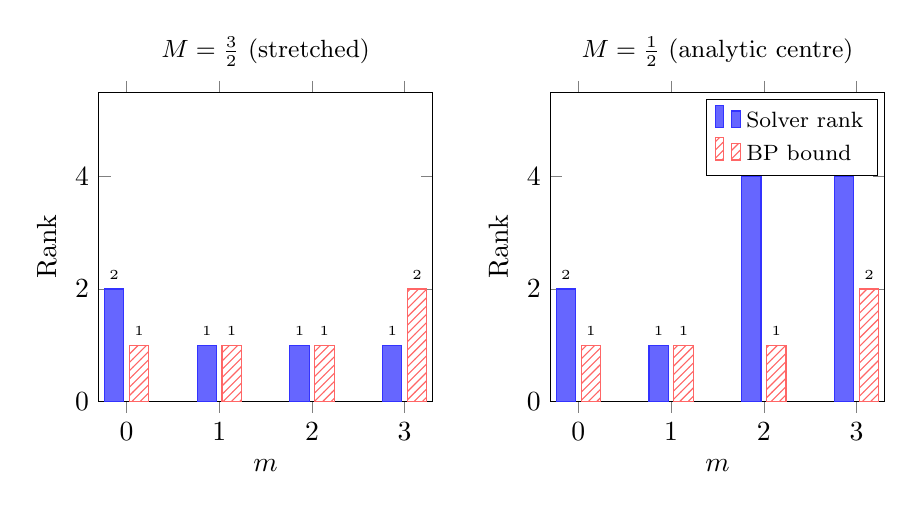
\begin{tikzpicture}
\begin{groupplot}[
    group style={
        group size=2 by 1,
        horizontal sep=1.5cm,
    },
    width=0.48\textwidth,
    height=5.5cm,
    ybar,
    /pgf/bar width=7pt,
    xlabel={$m$},
    ylabel={Rank},
    ymin=0, ymax=5.5,
    xtick={0,1,2,3},
    nodes near coords,
    every node near coord/.append style={font=\tiny},
]
\nextgroupplot[title={$M = \tfrac{3}{2}$ (stretched)}, title style={font=\small}]
\addplot[fill=blue!60, draw=blue!80] coordinates {
    (0, 2) (1, 1) (2, 1) (3, 1)
};
\addplot[fill=red!30, draw=red!60, pattern=north east lines, pattern color=red!60] coordinates {
    (0, 1) (1, 1) (2, 1) (3, 2)
};
\nextgroupplot[title={$M = \tfrac{1}{2}$ (analytic centre)}, title style={font=\small},
    legend style={at={(0.98,0.98)}, anchor=north east, font=\footnotesize},
    legend cell align=left]
\addplot[fill=blue!60, draw=blue!80] coordinates {
    (0, 2) (1, 1) (2, 4) (3, 4)
};
\addplot[fill=red!30, draw=red!60, pattern=north east lines, pattern color=red!60] coordinates {
    (0, 1) (1, 1) (2, 1) (3, 2)
};
\legend{Solver rank, BP bound}
\end{groupplot}
\end{tikzpicture}
\caption{Optimizer rank on the $n=2$ shell.
\textbf{Left:} $M=\tfrac{3}{2}$ (maximally stretched); the extreme-point
optimizer satisfies the BP bound $r \leq \lfloor\sqrt{m+1}\rfloor$.
\textbf{Right:} $M=\tfrac{1}{2}$; the interior-point solver converges to the
analytic centre of the optimal face (higher rank).  Facial reduction
would recover an extreme point satisfying BP.}
\label{fig:rank-vs-m}
\end{figure}

\begin{figure}[htbp]
\centering
\begin{tikzpicture}
\begin{axis}[
    width=0.85\textwidth,
    height=6cm,
    xlabel={Magnetic field strength $B$},
    ylabel={Optimal energy $E^*$},
    legend style={at={(0.02,0.98)}, anchor=north west, font=\small},
    legend cell align=left,
    grid=major,
    grid style={gray!30},
]
\addplot[blue, thick, mark=none]
    table[x index=0, y index=2] {../numerics/data/energy_vs_B_n3_m1.dat};
\addplot[red, thick, mark=none, dashed]
    table[x index=0, y index=2] {../numerics/data/energy_vs_B_n3_m2.dat};
\addplot[green!60!black, thick, mark=none, dotted, line width=1.5pt]
    table[x index=0, y index=2] {../numerics/data/energy_vs_B_n3_m3.dat};
\legend{$m=1$ ($J_z$), $m=2$ ($J_z{+}J^2$), $m=3$ ($J_z{+}J^2{+}L^2$)}
\end{axis}
\end{tikzpicture}
\caption{Optimal energy vs.\ field strength on the $n=3$ shell
($\dim=18$, $M=\tfrac{3}{2}$).  Adding constraints raises the minimum
energy.  All optimizers are pure ($r=1$), consistent with BP.}
\label{fig:energy-vs-B}
\end{figure}

\begin{figure}[htbp]
\centering
\begin{tikzpicture}
\begin{axis}[
    width=0.85\textwidth,
    height=6cm,
    xlabel={Hilbert space dimension $d = 2n^2$},
    ylabel={Rank of optimal $\rho^*$},
    ymin=0, ymax=55,
    xtick={8, 18, 32, 50},
    legend style={at={(0.02,0.98)}, anchor=north west, font=\small},
    legend cell align=left,
    grid=major,
    grid style={gray!30},
]
\addplot[blue, thick, mark=*, mark size=3pt]
    table[x index=1, y index=3] {../numerics/data/rank_vs_shell_m1.dat};
\addplot[red, thick, mark=square*, mark size=3pt]
    table[x index=1, y index=3] {../numerics/data/rank_vs_shell_m2.dat};
\addplot[green!60!black, thick, mark=triangle*, mark size=3pt]
    table[x index=1, y index=3] {../numerics/data/rank_vs_shell_m3.dat};
\addplot[gray, dashed, thick, mark=none, domain=5:55, samples=2] {x};
\addplot[blue!50, dotted, ultra thick, domain=5:55, samples=2] {1};
\addplot[green!60!black!50, dashdotted, thick, domain=5:55, samples=2] {2};
\legend{$m=1$, $m=2$, $m=3$,
        Na\"{\i}ve: $r \leq d$,
        BP ($m \leq 2$): $r \leq 1$,
        BP ($m = 3$): $r \leq 2$}
\end{axis}
\end{tikzpicture}
\caption{Optimizer rank vs.\ Hilbert space dimension ($B=1$,
$M=\tfrac{3}{2}$).  The rank stays at $1$ regardless of $d$, while the
na\"{\i}ve bound $r \leq d$ grows linearly.  For $n=5$ ($d=50$), BP
reduces the rank bound from $50$ to at most~$2$.}
\label{fig:rank-vs-dim}
\end{figure}

%% ========================================================================
\section{Cone-Valued Inequality Constraints}
\label{sec:conic-ineq}
%% ========================================================================

The results above treat scalar affine equality constraints
$\alpha_j(x) = b_j$.  A natural extension, proposed during the
follow-up discussion, is to allow \emph{conic inequality constraints}
where the constraint maps take values in ordered vector spaces.

\begin{theorem}[Barvinok--Pataki for conic inequalities]
\label{thm:conic-ineq}
Let $(V, V^+)$ be an ordered vector space with pointed cone, and let
$I$ be a finite index set.  For each $i \in I$, let $(W_i, W_i^+)$
be an ordered vector space and $\Phi_i \colon V \to W_i$ a linear map.
For given $a_i \in W_i$, define the feasible set
\[
  C = \bigl\{\, x \in V^+ \;\big|\;
    \Phi_i(x) \geq_{W_i^+} a_i \;\;\forall\, i \in I \,\bigr\},
\]
where $\Phi_i(x) \geq_{W_i^+} a_i$ means
$\Phi_i(x) - a_i \in W_i^+$.  Set $m = \sum_{i \in I} \dim(W_i)$.
If $x$ is an extreme point of $C$ and
$d_F = \dim(\spn(\face_{V^+}(x)))$ is finite, then
\[
  \boxed{\; d_F \;\leq\; m. \;}
\]
\end{theorem}

\begin{proof}
Define the combined constraint map
$\Phi \colon V \to \bigoplus_{i} W_i$ by
$\Phi(v) = (\Phi_i(v))_{i \in I}$.  Let
$F = \face_{V^+}(x)$ and consider the restriction
$\Phi_F \colon \spn(F) \to \bigoplus_i W_i$.

By rank--nullity,
$d_F = \dim(\ker\Phi_F) + \dim(\im\Phi_F)
     \leq \dim(\ker\Phi_F) + m$.

It suffices to show $\ker\Phi_F = \{0\}$ when $x$ is extreme in $C$.
Suppose $D \in \ker\Phi_F$, $D \neq 0$.  Then $\Phi_i(D) = 0$ for
all $i$, so
\[
  \Phi_i(x + tD) - a_i
  = (\Phi_i(x) - a_i) + t\,\Phi_i(D)
  = \Phi_i(x) - a_i \in W_i^+
\]
for all $t \in \R$.  Hence $x + tD$ satisfies all conic inequality
constraints whenever $x + tD \in V^+$.  The remainder of the argument
(perturbation along $D$, exit from $V^+$ by pointedness,
contradiction with extremality) follows identically to
Steps~2--4 of Theorem~\ref{thm:general}.
\end{proof}

\begin{remark}[Equality vs.\ inequality constraints]
\label{rmk:eq-vs-ineq}
\leavevmode
\begin{enumerate}
\item \textbf{Equalities.}
  If the constraints are equalities $\Phi_i(x) = a_i$, each
  can be decomposed into $\dim(W_i)$ scalar equalities and
  the bound $d_F \leq m$ reduces to Theorem~\ref{thm:general}.

\item \textbf{Simplex cones ($W_i^+ \cong \R_+^{k_i}$).}
  A conic inequality $\Phi_i(x) \geq_{\R_+^{k_i}} a_i$ is
  equivalent to $k_i$ scalar inequality constraints.  The conic
  bound $d_F \leq \sum k_i$ coincides with the scalar bound.

\item \textbf{Non-simplex cones (e.g.\ $W_i^+ = \PSD_{k_i}$).}
  The conic bound $d_F \leq \sum \dim(\Sym_{k_i})$ cannot be
  recovered by converting each inequality to scalar constraints,
  because the PSD cone is not generated by a simplex.

\item \textbf{Inactive constraints.}
  If a conic constraint is \emph{inactive} at $x$ (i.e.\
  $\Phi_i(x) - a_i$ lies in the interior of $W_i^+$), then any
  perturbation $D$ preserves this constraint for small $|t|$,
  regardless of $\Phi_i(D)$.  Thus inactive constraints do not
  contribute to the kernel condition.  More precisely, if $k$
  constraints are inactive, then $d_F \leq m'$ where
  $m' = \sum_{i:\, \text{active}} \dim(W_i)$.
\end{enumerate}
\end{remark}

\begin{remark}[Slack variable formulation]
\label{rmk:slack}
Alternatively, one can introduce slack variables
$S_i = \Phi_i(x) - a_i \in W_i^+$ and rewrite the conic
inequality as an equality $\Phi_i(x) - S_i = a_i$ over the
product cone $V^+ \times \prod_i W_i^+$.  The face of the product
cone at $(x, (S_i)_i)$ has dimension
$d_F(x) + \sum_i d_F(S_i \text{ in } W_i^+)$, and the equality
formulation gives
\[
  d_F(x) + \sum_{i} d_F(S_i) \;\leq\; \sum_i \dim(W_i).
\]
This is at least as tight as Theorem~\ref{thm:conic-ineq}
whenever some slack $S_i$ has a non-trivial face (i.e.\ the
constraint is not fully active).  However, the slack formulation
requires tracking the face structure of each $S_i$, which may
not be accessible a priori.  Moreover, practical face-reduction
algorithms (iterating the perturbation argument) cannot control
whether they reduce $d_F(x)$ or $d_F(S_i)$ at each step.
\end{remark}

\subsection{Numerical verification: compression constraint}

We illustrate Theorem~\ref{thm:conic-ineq} and
Remark~\ref{rmk:slack} with a concrete example: $X \in \PSD_8$
(real symmetric, $8 \times 8$) subject to $m_s$ scalar equality
constraints and a $3 \times 3$ conic inequality
$P^\top X P \succeq B$, where $P$ is the projection onto the
first 3 coordinates and $B$ is a fixed rank-$2$ PSD matrix.
The conic inequality contributes $\dim(\Sym_3) = 6$ to the
constraint count, so Martin's bound gives
$r(r{+}1)/2 \leq m_s + 6$ and Lennart's slack bound gives
$r(r{+}1)/2 \leq m_s + 6 - r_S(r_S{+}1)/2$,
where $r_S = \rank(P^\top X P - B)$.

\begin{table}[htbp]
\centering
\caption{PSD constraint on a $3 \times 3$ subblock of
$X \in \PSD_8$.  ``No LMI'' uses only $m_s$ scalar equalities.
``Martin'' adds the conic constraint dimension.  ``Lennart''
subtracts the slack face dimension.  In all cases the slack
has rank~1, so Lennart's bound is marginally tighter.}
\label{tab:compression}
\begin{tabular}{ccccccc}
\toprule
$m_s$ & \multicolumn{2}{c}{\textbf{No LMI}}
  & \multicolumn{2}{c}{\textbf{Martin}}
  & \multicolumn{2}{c}{\textbf{Lennart ($r_S = 1$)}} \\
\cmidrule(lr){2-3}\cmidrule(lr){4-5}\cmidrule(lr){6-7}
  & $r$ & bound & $r$ & bound & $r$ & bound \\
\midrule
1 & 1 & $\leq 1$ & 3 & $\leq 3$ & 3 & $\leq 3$ \\
3 & 1 & $\leq 2$ & 3 & $\leq 3$ & 3 & $\leq 3$ \\
5 & 2 & $\leq 2$ & 3 & $\leq 4$ & 3 & $\leq 4$ \\
8 & 3 & $\leq 3$ & 3 & $\leq 4$ & 3 & $\leq 4$ \\
\bottomrule
\end{tabular}
\end{table}

\noindent
The ``No LMI'' column shows that without the subblock constraint,
the optimizer has low rank (standard BP).  Adding the conic
inequality allows higher-rank optimizers (the feasible set is
larger), and the rank is correctly bounded by both Martin's and
Lennart's formulations.  The slack $S = P^\top X^* P - B$
consistently has rank~1, making the two bounds coincide at
$r(r{+}1)/2 \leq m_s + 5$.

%% ========================================================================
\section{Application to Spectrahedra}
\label{sec:spectrahedra}
%% ========================================================================

A \emph{spectrahedron} is the feasible set of a semidefinite program,
typically defined by one or more linear matrix inequalities (LMIs).
Theorem~\ref{thm:conic-ineq} applies directly.

\begin{corollary}[Block-diagonal LMI spectrahedra]
\label{cor:block-lmi}
Let $x \in \R^n$ and consider two LMI constraints
\[
  F(x) = F_0 + \textstyle\sum_{i=1}^n x_i F_i \succeq 0, \qquad
  G(x) = G_0 + \textstyle\sum_{i=1}^n x_i G_i \succeq 0,
\]
with $F_i \in \Sym_k$, $G_i \in \Sym_p$.  If $x^*$ is an extreme
point of the spectrahedron $S = \{x : F(x) \succeq 0,\, G(x) \succeq 0\}$,
then
\[
  \frac{(r_F + r_G)(r_F + r_G + 1)}{2} \;\leq\; n,
\]
where $r_F = \rank(F(x^*))$ and $r_G = \rank(G(x^*))$.  This is
strictly tighter than the individual bounds
$r_F(r_F+1)/2 \leq n$ and $r_G(r_G+1)/2 \leq n$.
\end{corollary}

\begin{proof}
The combined LMI $\operatorname{diag}(F(x), G(x)) \succeq 0$ is a
single $(k{+}p) \times (k{+}p)$ LMI parameterised by $n$ variables.
The standard Barvinok--Pataki bound gives the result.  The tightening
over individual bounds follows from $(r_F + r_G)^2 > r_F^2 + r_G^2$
when both ranks are positive.
\end{proof}

\subsection{Numerical verification: block-diagonal LMI}

We generate a random spectrahedron with $n = 10$ free variables,
two $4 \times 4$ LMI blocks $F(x) \succeq 0$ and $G(x) \succeq 0$,
and two trace equality constraints
$\Tr(F(x)) = \Tr(F_0)$, $\Tr(G(x)) = \Tr(G_0)$ for compactness.
The individual BP bound gives $r_F \leq 4$ and $r_G \leq 4$
(since $r(r{+}1)/2 \leq 12$ yields $r \leq 4$), while the
block-diagonal bound gives
$(r_F + r_G)(r_F + r_G + 1)/2 \leq 10$, i.e.\
$r_F + r_G \leq 4$.

Table~\ref{tab:block-lmi} shows results from 8 random
perturbations of the objective (to generically select distinct
extreme points of the optimal face).  The interior-point solver
(Mosek) returns the analytic centre, which may have higher
combined rank than a true extreme point; trials marked $\checkmark$
satisfy the block-diagonal bound.

\begin{table}[htbp]
\centering
\caption{Block-diagonal LMI spectrahedron ($n = 10$, two
$4 \times 4$ blocks, 2 trace equalities).  The individual bound
$r_F, r_G \leq 4$ holds in all trials; the tighter combined bound
$r_F + r_G \leq 4$ holds at extreme points (5 of 8 trials).
Trials with $r_F + r_G = 5$ correspond to the analytic centre,
not an extreme point.}
\label{tab:block-lmi}
\begin{tabular}{ccccc}
\toprule
\textbf{Trial} & $r_F$ & $r_G$ & $r_F + r_G$
  & \textbf{Combined BP} \\
\midrule
1 & 3 & 2 & 5 & $\times$ \\
2 & 2 & 2 & 4 & $\checkmark$ \\
3 & 2 & 2 & 4 & $\checkmark$ \\
4 & 2 & 2 & 4 & $\checkmark$ \\
5 & 3 & 2 & 5 & $\times$ \\
6 & 2 & 2 & 4 & $\checkmark$ \\
7 & 3 & 2 & 5 & $\times$ \\
8 & 2 & 2 & 4 & $\checkmark$ \\
\bottomrule
\end{tabular}
\end{table}

\subsection{Application: entanglement witness rank bound}

\begin{example}[Entanglement witness rank bound]
\label{ex:witness}
Let $d = d_A \cdot d_B$ and consider the cone of PPT
(positive partial transpose) matrices:
\[
  \mathcal{P} = \bigl\{\, W \in \PSD_d \;\big|\;
    W^{\Gamma_B} \succeq 0 \,\bigr\},
\]
where $\Gamma_B$ denotes partial transpose on subsystem $B$.
This is a pointed closed cone (if $W, -W \in \mathcal{P}$, then
$W = 0$).  The constraint $W^{\Gamma_B} \succeq 0$ is a conic
inequality with $\Phi = \Gamma_B$, $W_1^+ = \PSD_d$,
$\dim(W_1) = d(d+1)/2$ (real) or $d^2$ (complex Hermitian).

Consider optimising over $\mathcal{P}$ subject to $m$ scalar
affine constraints (e.g.\ normalisation $\Tr(W) = 1$ and
$\Tr(A_j W) = b_j$).  By Theorem~\ref{thm:conic-ineq}, any
extreme point $W^*$ satisfies
\[
  \rank(W^*)^2 \;\leq\; m \quad\text{and}\quad
  \rank(W^{*\Gamma_B})^2 \;\leq\; m,
\]
where the first bound comes from the face of $\PSD_d$ and the
second from the face of the PPT cone.

For $m = 1$ (normalisation only): $\rank(W^*) = 1$ and
$\rank(W^{*\Gamma_B}) = 1$.  The extreme PPT witnesses under
normalisation alone are rank-$1$ with rank-$1$ partial transpose,
i.e.\ they are product projectors $\ket{\psi}\bra{\psi} \otimes
\ket{\phi}\bra{\phi}$.
\end{example}

We verify the witness rank bound numerically for
$d_A = d_B = 2$ ($d = 4$), optimising $\Tr(W\rho_{\text{target}})$
over the PPT cone $\{W \succeq 0 : W^{\Gamma_B} \succeq 0\}$
with $m$ affine constraints.  Results are shown in
Table~\ref{tab:ppt-witness}.  As $m$ increases, the ranks of
$W$ and $W^{\Gamma}$ grow, but $\rank(W^{\Gamma})$ stays bounded
by $\lfloor\sqrt{m+1}\rfloor$ (the PPT-cone BP bound).
At $m = 8$, $W$ has full rank~4 while $W^{\Gamma}$ has rank~3,
illustrating that the conic constraint controls the partial-transpose
rank independently.

\begin{table}[htbp]
\centering
\caption{PPT entanglement witness for a $2 \times 2$ system
($d = 4$).  The BP bound from the PPT cone gives
$\rank(W^{\Gamma}) \leq \lfloor\sqrt{m+1}\rfloor$; the PSD
face gives $\rank(W) \leq \lfloor\sqrt{m+1}\rfloor$.
Eigenvalues listed in decreasing order.}
\label{tab:ppt-witness}
\begin{tabular}{ccccl}
\toprule
$m$ & $\rank(W)$ & $\rank(W^{\Gamma})$
  & $\Tr(W\rho)$ & \textbf{Eigenvalues of $W$} \\
\midrule
1 & 2 & 2 & $0.000$ & $(2.519,\; 1.481,\; 0,\; 0)$ \\
2 & 2 & 2 & $0.019$ & $(2.605,\; 1.395,\; 0,\; 0)$ \\
4 & 3 & 3 & $0.521$ & $(3.515,\; 0.462,\; 0.023,\; 0)$ \\
8 & 4 & 3 & $0.562$ & $(2.120,\; 1.208,\; 0.589,\; 0.083)$ \\
\bottomrule
\end{tabular}
\end{table}

%% ========================================================================
\section{Inequality Constraints and the Role of Slack}
\label{sec:inequality}
%% ========================================================================

The interplay between equality and inequality constraints merits
further discussion, following observations by Lennart Binkowski
and Timo Ziegler.

\begin{example}[PSD matrix with scalar inequalities]
\label{ex:scalar-ineq}
Consider $X \in \PSD_n$ (real symmetric) with $m$ scalar inequality
constraints $\Tr(A_i X) \leq b_i$.  Introducing slack variables
$s_i \geq 0$ with $\Tr(A_i X) + s_i = b_i$, this becomes a problem
over the product cone $\PSD_n \times \R_+^m$ with $m$ equality
constraints.

The face of the product cone at $(X, s)$ has dimension
\[
  d_F(X, s) = \frac{r(r+1)}{2} + |\{i : s_i > 0\}|,
\]
where $r = \rank(X)$.  The Barvinok--Pataki bound gives
\begin{equation}\label{eq:slack-bound}
  \frac{r(r+1)}{2} + |\{i : s_i > 0\}| \;\leq\; m.
\end{equation}
In particular, if all constraints are active ($s_i = 0$ for all
$i$), then $r(r+1)/2 \leq m$ (the equality-constraint bound).
If $k$ constraints are inactive, then
$r(r+1)/2 \leq m - k$, confirming the heuristic that inactive
constraints ``free up'' dimensions.

However, a face-reduction algorithm iterating the perturbation
argument of Theorem~\ref{thm:general} cannot guarantee which
term in \eqref{eq:slack-bound} decreases at each step: it may
reduce $\rank(X)$ or merely set some $s_i$ to zero.
\end{example}

We verify \eqref{eq:slack-bound} numerically for
$X \in \PSD_6$ (real symmetric) with $m$ random scalar inequality
constraints $\Tr(A_i X) \leq b_i$ and the normalisation
$\Tr(X) = 1$ (one equality, counted separately).  Table~\ref{tab:ineq-slack} shows that the combined face dimension
$r(r{+}1)/2 + |\{s_i > 0\}|$ saturates the bound $m + 1$ at
$m = 15$, and that the effective rank bound from counting only
active constraints (Remark~\ref{rmk:eq-vs-ineq}(4)) is
consistently satisfied.

\begin{table}[htbp]
\centering
\caption{Scalar inequality constraints on $\PSD_6$
($\Tr(X) = 1$).  The combined face dimension
$d_F = r(r{+}1)/2 + |\{s_i > 0\}|$ satisfies $d_F \leq m + 1$
(the $+1$ from the trace equality).  At $m = 15$,
the bound is \emph{tight}: $d_F = 16 = m + 1$.}
\label{tab:ineq-slack}
\begin{tabular}{cccccccc}
\toprule
$m$ & $\rank$ & $\frac{r(r{+}1)}{2}$ & Active & Inactive
  & $d_F$ & Bound & \\
\midrule
 3 & 1 & 1 & 1 & 2 &  3 &  4 & $\checkmark$ \\
 6 & 1 & 1 & 0 & 6 &  7 &  7 & \textbf{tight} \\
10 & 1 & 1 & 3 & 7 &  8 & 11 & $\checkmark$ \\
15 & 2 & 3 & 2 & 13 & 16 & 16 & \textbf{tight} \\
\bottomrule
\end{tabular}
\end{table}

\noindent
The column ``Active'' is $|\{i : s_i = 0\}|$.  By the
inactive-constraint reduction, $r(r{+}1)/2 \leq
(\text{active constraints}) + 1$: for $m = 15$ this gives
$r(r{+}1)/2 \leq 3$, hence $r \leq 2$, matching the observed
$\rank(X^*) = 2$.

%% ========================================================================
\section{Obstructions to Nonlinear Extensions}
\label{sec:nonlinear}
%% ========================================================================

It is natural to ask whether the Barvinok--Pataki bound extends to
nonlinear constraints.  Two perspectives emerged from the discussion.

\begin{remark}[Manifold framework]
If the equality constraints involve smooth nonlinear functions
$f_i \colon V \to \R$ and the target values $(b_1, \ldots, b_m)$
are regular values, then by the implicit function theorem the
constraint set $C = \{x \in V^+ : f_i(x) = b_i\}$ is a smooth
manifold of codimension $m$.  The perturbation direction $D$ lives
in the kernel of the differential $Df|_x$ restricted to the tangent
cone of $V^+$ at $x$.  The rank--nullity argument applies to the
differential, giving a \emph{local} dimension bound.

However, it is not clear whether the resulting flow
$t \mapsto x + tD + O(t^2)$ reaches a face of $V^+$ of strictly
lower dimension, which is the analogue of Step~3 in the proof of
Theorem~\ref{thm:general}.
\end{remark}

\begin{remark}[Obstruction to localisation]
The Barvinok--Pataki argument fundamentally relies on
\emph{linearity} of the constraints: the perturbation $x + tD$
preserves the constraint \emph{exactly} (not merely to first
order), so the entire line segment from $x$ to the boundary of
$V^+$ is feasible.

For nonlinear constraints, this fails.  A nonlinear constraint
can force a feasible point to lie deep in the interior of a
high-dimensional face, with no feasible path to the boundary.
For example, consider a polyhedron $P$ with a nonlinear constraint
that confines $x$ to a ``shell'' strictly inside $P$: every
point satisfying the constraint is interior to $P$, so no
perturbation reaches a proper face.

Linear constraints avoid this because they generate faces upon
intersection with the cone: the hyperplane $\{x : \alpha(x) = b\}$
slices the cone into proper faces.
\end{remark}

%% ========================================================================
\section{Infinite-Dimensional Example: The Cuntz Algebra $\mathcal{O}_2$}
\label{sec:cuntz}
%% ========================================================================

We illustrate the infinite-dimensional theory with the Cuntz algebra
$\mathcal{O}_2$, a C$^*$-algebra that is fundamentally different from
$B(\mathcal{H})$: it is simple, purely infinite, admits \emph{no}
tracial states, and has \emph{no} finite-dimensional representations.
Nevertheless, the Barvinok--Pataki bound applies and yields strong
structural results.

\subsection{The Cuntz algebra $\mathcal{O}_n$}

The \emph{Cuntz algebra} $\mathcal{O}_n$ ($n \geq 2$) is the
universal C$^*$-algebra generated by $n$ isometries
$S_1, \ldots, S_n$ satisfying
\[
  S_i^* S_j = \delta_{ij}\, \id, \qquad
  \sum_{i=1}^n S_i S_i^* = \id.
\]
Key properties \cite{cuntz77}:
\begin{enumerate}
\item \textbf{Simple:} $\mathcal{O}_n$ has no non-trivial closed
  two-sided ideals.  Every representation is faithful.
\item \textbf{Purely infinite:} every non-zero hereditary
  C$^*$-subalgebra contains an infinite projection.
\item \textbf{No tracial states:} if $\tau$ were a trace, then
  $1 = \tau(\id) = \sum_i \tau(S_i S_i^*) = \sum_i \tau(S_i^* S_i)
  = n \cdot \tau(\id) = n$, a contradiction.
\item \textbf{No finite-dimensional representations:} any such
  would induce a trace via the normalised matrix trace.
\end{enumerate}

The \emph{gauge action} $\gamma_z(S_i) = z\, S_i$ ($z \in \mathbb{T}$)
has fixed-point algebra $\mathcal{O}_n^{\mathbb{T}} \cong
M_{n^\infty}$ (the UHF algebra of type $n^\infty$), which is the
norm closure of $\bigcup_{k=0}^\infty M_{n^k}(\mathbb{C})$ embedded
via the canonical shifts.

\subsection{States and symbolic dynamics}

A state $\varphi$ on $\mathcal{O}_n$ restricts to a probability
measure on the Cantor space $\{1, \ldots, n\}^{\mathbb{N}}$ via
the \emph{diagonal subalgebra}
$\mathcal{D}_n = C^*(\{S_\mu S_\mu^* : \mu \in \{1,\ldots,n\}^*\})
\cong C(\{1,\ldots,n\}^{\mathbb{N}})$.
The cylinder probabilities are
\[
  p(\mu) = \varphi(S_\mu S_\mu^*),
\]
where $S_\mu = S_{\mu_1} \cdots S_{\mu_k}$ for a finite word
$\mu = \mu_1 \cdots \mu_k$.  The Cuntz relation ensures consistency:
$\sum_{i=1}^n p(\mu i) = p(\mu)$.

\emph{Bernoulli states} ($\varphi(S_\mu S_\mu^*) =
\prod_j p_{\mu_j}$ for a probability vector $(p_1, \ldots, p_n)$)
are \textbf{pure}: the GNS representation is irreducible.  \emph{Markov
states} (determined by a stochastic matrix $P$ and its stationary
distribution $\pi$, with
$\varphi(S_\mu S_\mu^*) = \pi_{\mu_1} P_{\mu_1\mu_2} \cdots
P_{\mu_{k-1}\mu_k}$) are generally \textbf{not pure}: for an
irreducible aperiodic chain, the GNS representation yields a
type~III factor \cite{bratteli_jorgensen99}.

\subsection{Barvinok--Pataki for $\mathcal{O}_n$}

\begin{corollary}[BP for Cuntz algebras]\label{cor:cuntz-bp}
Let $a_1, \ldots, a_m \in (\mathcal{O}_n)_\sa$ and
$b_1, \ldots, b_m \in \R$.  Define
\[
  C = \bigl\{\, \varphi \in S(\mathcal{O}_n) \;\big|\;
    \varphi(a_j) = b_j,\; j = 1, \ldots, m \,\bigr\}.
\]
If $\varphi$ is an extreme point of $C$, then the commutant
$\pi_\varphi(\mathcal{O}_n)'$ is finite-dimensional, with
\[
  \dim_\R\bigl(\pi_\varphi(\mathcal{O}_n)'\bigr)_\sa
  \;\leq\; m + 1.
\]
In particular, the GNS representation $\pi_\varphi$ is
\textbf{type~I} (a direct sum of finitely many irreducible
representations with finite multiplicities), despite the fact
that generic states on $\mathcal{O}_n$ yield type~III factors.
\end{corollary}

\begin{proof}
By Corollary~\ref{cor:cstar} (which applies to any unital
C$^*$-algebra, including simple purely infinite ones).  The
conclusion that $\pi_\varphi$ is type~I follows from the
finite-dimensionality of the commutant: if
$\pi_\varphi(\mathcal{O}_n)' \cong \bigoplus_j M_{n_j}(\mathbb{C})$
with $\sum n_j^2 \leq m + 1$, then $\pi_\varphi$ decomposes
into at most $m + 1$ irreducible summands with finite multiplicities.
\end{proof}

\begin{remark}[Type collapse]
This is a strong structural result.  A generic state on
$\mathcal{O}_n$ (e.g.\ a Markov state from an aperiodic chain)
gives a type~III factor representation, where the commutant is
an infinite-dimensional type~III factor.  The BP bound says that
finitely many affine constraints force the extreme states to
``collapse'' from type~III to type~I.  The number of constraints
$m$ controls the complexity of the type~I decomposition:
\begin{center}
\begin{tabular}{clc}
\toprule
$m$ & \textbf{Commutant structure} & \textbf{Decomposition} \\
\midrule
$0$ & $\mathbb{C}$ & Pure state \\
$1$ & $\mathbb{C}$ or $\mathbb{C} \oplus \mathbb{C}$
  & Pure, or mixture of 2 irreducibles \\
$3$ & $\leq M_2(\mathbb{C})$
  & Irreducible with multiplicity $\leq 2$ \\
$m$ & $\bigoplus_j M_{n_j}(\mathbb{C})$, $\sum n_j^2 \leq m+1$
  & Controlled multiplicity \\
\bottomrule
\end{tabular}
\end{center}
\end{remark}

\subsection{Numerical verification via truncation}

Since $\mathcal{O}_2$ has no finite-dimensional representations,
we approximate by \emph{truncation}: the gauge-invariant subalgebra
$\mathcal{O}_2^{\mathbb{T}} \cong M_{2^\infty}$ contains the
finite-level algebras $M_{2^L}$, and gauge-invariant states
restrict to density matrices $\rho_L \in \PSD_{2^L}$.  The
constraint $\varphi(S_\mu S_\mu^*) = p_\mu$ becomes
$\Tr(P_\mu \rho_L) = p_\mu$, where $P_\mu$ is the projection
onto words of length $L$ extending $\mu$.

We solve the truncated SDP on $M_{2^L}$ with $m$ gauge-invariant
constraints and verify the BP bound $r^2 \leq m + 1$ (complex case)
at each level.

\paragraph{Gauge-invariant constraints on $\mathcal{O}_2$.}

Table~\ref{tab:cuntz-gauge} shows optimiser ranks for
$\mathcal{O}_2$ truncated to level $L = 4$ ($d = 16$) with
increasing numbers of ``word'' constraints
$\varphi(S_\mu S_\mu^*) = p_\mu$.  With few constraints
($m \leq 8$), all optimisers are pure (rank~1); this reflects
the abundance of pure states on $\mathcal{O}_2$ (every
Bernoulli state is pure).  At $m = 15$ (all cylinder
probabilities through depth~3, from a non-Bernoulli Markov chain),
the optimiser becomes rank~2 --- a genuinely mixed state
with eigenvalues $(0.894, 0.106)$.

\begin{table}[htbp]
\centering
\caption{Gauge-invariant constraints on $\mathcal{O}_2$, truncated
to $M_{16}$ ($L = 4$).  Constraints are cylinder probabilities
$\varphi(S_\mu S_\mu^*) = p_\mu$ for words of increasing depth.
The last row uses values from a Markov chain with
$P = \bigl[\begin{smallmatrix}0.4 & 0.6 \\ 0.35 & 0.65
\end{smallmatrix}\bigr]$, which is non-Bernoulli.}
\label{tab:cuntz-gauge}
\begin{tabular}{ccccl}
\toprule
$m$ & Depth & $\rank(\rho^*_L)$ & BP bound
  & \textbf{Leading eigenvalues} \\
\midrule
 2 & 1 & 1 & $\leq 1$ & $(1)$ \\
 3 & 1--2 & 1 & $\leq 1$ & $(1)$ \\
 5 & 1--2 & 1 & $\leq 2$ & $(1)$ \\
 8 & 1--3 & 1 & $\leq 2$ & $(1)$ \\
15 & 1--3 (Markov) & \textbf{2} & $\leq 3$ & $(0.894,\; 0.106)$ \\
\bottomrule
\end{tabular}
\end{table}

\paragraph{Convergence with truncation level.}

Table~\ref{tab:cuntz-conv} shows that the optimiser rank is
\emph{stable} as $L$ increases from~2 to~6
($d$ from~4 to~64): the rank stays at~1 for all levels.
This is consistent with the full $\mathcal{O}_2$ result
(Corollary~\ref{cor:cuntz-bp}), which gives the same bound
independently of the Hilbert space dimension.

\begin{table}[htbp]
\centering
\caption{Rank stability with truncation level $L$.  Fixed constraints:
$\varphi(S_1 S_1^*) = 0.3$, $\varphi(S_{11} S_{11}^*) = 0.15$,
$\varphi(S_{12} S_{12}^*) = 0.15$, $\varphi(S_{21} S_{21}^*) = 0.25$
($m = 5$, BP bound $r \leq 2$).}
\label{tab:cuntz-conv}
\begin{tabular}{cccc}
\toprule
$L$ & $\dim = 2^L$ & $\rank(\rho^*_L)$ & BP bound \\
\midrule
2 &  4 & 1 & $\leq 2$ \\
3 &  8 & 1 & $\leq 2$ \\
4 & 16 & 1 & $\leq 2$ \\
5 & 32 & 1 & $\leq 2$ \\
6 & 64 & 1 & $\leq 2$ \\
\bottomrule
\end{tabular}
\end{table}

\paragraph{Markov constraints forcing mixed states.}

A \emph{Bernoulli($p$)} state satisfies
$\varphi(S_1^k (S_1^*)^k) = p^k$ for all $k$.  Deviating from
this product structure (setting
$\varphi(S_1^2(S_1^*)^2) = q \neq p^2$) forces non-Bernoulli
states.  With only $m = 3$ constraints (trace, $p$, and $q$),
the BP bound gives $r^2 \leq 3$, so $r = 1$; indeed, all
optimisers are pure for all tested values of $q$.  Mixed states
arise only when the number of constraints exceeds the number of
``degrees of freedom'' of the pure state manifold.

For Markov-chain constraints at depth~3 ($m = 15$ constraints
from a non-Bernoulli transition matrix), the optimiser has
rank~2, saturating neither the BP bound ($r \leq 3$) nor the
na\"{\i}ve bound ($r \leq 16$), but demonstrating that the
infinite-dimensional Cuntz algebra structure reduces to a
finite-rank problem under finitely many constraints.

\subsection{Physical and mathematical significance}

The Cuntz algebra example highlights three features of the
generalised Barvinok--Pataki theorem:

\begin{enumerate}
\item \textbf{No density matrices needed.}  The state space of
  $\mathcal{O}_n$ has no density matrix description (no traces),
  yet the BP bound controls the face dimension and hence the
  commutant structure.  This is a purely convex-geometric result,
  not an operator-algebraic one.

\item \textbf{Type collapse.}  Finitely many affine constraints
  force extreme states from type~III (generic for $\mathcal{O}_n$)
  to type~I (finite-dimensional commutant).  The number of
  constraints controls the complexity of the decomposition.

\item \textbf{Truncation stability.}  The BP bound is independent
  of the Hilbert space dimension.  Numerically, the truncation
  $\mathcal{O}_n \hookrightarrow M_{n^L}$ gives consistent ranks
  as $L \to \infty$, confirming that the finite-dimensional
  approximation captures the full infinite-dimensional structure.
\end{enumerate}

%% ========================================================================
\section*{Acknowledgements}
%% ========================================================================

The proof idea underlying this work is due to Timo Ziegler, who
presented the classical Barvinok--Pataki argument for PSD matrices
during a blackboard discussion at the Institut f\"ur Theoretische
Physik, Leibniz Universit\"at Hannover, on 3 March 2026.  His
formulation of the perturbation--extremality argument was
subsequently recognised to generalise directly to pointed cones
and Archimedean order unit spaces.  Martin Plavala recognised during the discussion that the
argument extends to general cones.  Alexander Stottmeister
pointed out that the face-dimension quantity $d_F$ can be controlled
in infinite dimensions via Theorem~3.3 of Weis--Shirokov
\cite{weis_shirokov21}, which requires only a real vector space and
a convex set, without operator-algebraic assumptions.  The recording
was transcribed and typeset with the assistance of Claude (Anthropic).

\begin{thebibliography}{9}
\bibitem{barvinok02}
  A.~Barvinok,
  \emph{A Course in Convexity},
  Graduate Studies in Mathematics, vol.~54, AMS, 2002.

\bibitem{pataki98}
  G.~Pataki,
  On the rank of extreme matrices in semidefinite programs and the
  multiplicity of optimal eigenvalues,
  \emph{Math.\ Oper.\ Res.}\ \textbf{23}(2), 339--358, 1998.

\bibitem{alfsen_shultz03}
  E.M.~Alfsen and F.W.~Shultz,
  \emph{Geometry of State Spaces of Operator Algebras},
  Birkh\"auser, 2003.

\bibitem{weis_shirokov21}
  S.~Weis and M.E.~Shirokov,
  The face generated by a point, generalized affine constraints, and
  quantum theory,
  \emph{J.\ Convex Anal.}\ \textbf{28}(3), 847--870, 2021.
  arXiv:2003.14302.

\bibitem{rockafellar70}
  R.T.~Rockafellar,
  \emph{Convex Analysis},
  Princeton University Press, 1970.

\bibitem{cuntz77}
  J.~Cuntz,
  Simple C$^*$-algebras generated by isometries,
  \emph{Comm.\ Math.\ Phys.}\ \textbf{57}(2), 173--185, 1977.

\bibitem{bratteli_jorgensen99}
  O.~Bratteli and P.E.T.~Jorgensen,
  \emph{Iterated Function Systems and Permutation Representations
  of the Cuntz Algebra},
  Memoirs of the AMS, vol.~139, no.~663, 1999.
\end{thebibliography}

\end{document}
